\documentclass[supercite]{HustGraduPaper}
%进行个人信息设置
\title{多传感器融合技术}
\author{杨金昊} %作者姓名
\date{\today} %日期,默认当日
\school{自动化学院} %院系名称
\classnum{自卓1601} %专业班级
\stunum {U201614480} %学号
\instructor{张朴} %指导教师姓名

%添加自己要用的其他宏包
\usepackage{xltxtra}
\usepackage{listings}
\usepackage{bm}
\usepackage{tabularx}
\usepackage{multirow}
\usepackage{graphicx}
\usepackage{float}

\lstset{numbers=left,
language=matlab, basicstyle=\small,
numberstyle=\tiny,
keywordstyle=\color{blue!70}, 
commentstyle=\color{red!50!green!50!blue!50},
frame=shadowbox,
rulesepcolor=\color{red!20!green!20!blue!20},
breaklines=true
}


\begin{document}
	%生成标题页 \maketitle[可选参数]
	%可选参数:
	%logo color=green/black 华中科技大学字样的颜色,绿色或者黑色,默认绿色
	%line length=12em 填写信息处横线的长度,默认12em
	%line font=huawenzhongsong 填写信息的字体,默认huawenzhongsong
	\maketitle[logo color= black]

	\clearpage %结束上一页
	\pagenumbering{Roman} %摘要页码为大写罗马数字

	\tableofcontents
	
	%生成目录 \tableofcontents[可选参数]
	%可选参数:
	%pagenum=yes/no/true/false 目录是否显示页码,默认为false
	%toc in toc=yes/no/true/false 目录中是否有目录及其页码,默认为false
	%level=4 目录级数,默认是4,即显示到subsubsubsection
	%section indent=0em 目录第一级的缩进,默认是0em
	%subsection indent=1.5em 目录第二级的缩进,默认是1.5em
	%subsubsection indent=3.8em 目录第三级的缩进,默认是3.8em
	%subsubsubsection indent=7em 目录第四级的缩进,默认是7em
	%paragraph indent=11em 目录第五级的缩进,默认是11em
	%subparagraph indent=13em 目录第六级的缩进,默认13em
	%indent=normal/noindent/hustnoindent/sameforsubandsubsub 快速缩进设置,具体见文档
	%dot sep=4.5 目录点间距,默认4.5
	%section dot sep=4.5 目录第一级的点间距,默认是4.5
	%subsection dot sep=4.5 目录第二级的点间距,默认是4.5
	%subsubsection dot sep=4.5 目录第三级的点间距,默认是4.5
	%subsubsubsection dot sep=4.5 目录第四级的点间距,默认是4.5
	%paragraph dot sep=4.5 目录第五级的点间距,默认是4.5
	%subparagraph dot sep=4.6 目录第六级的点间距,默认是4.5
	%请注意在合适的位置放置\pagenumbering{numstyle}使用新的页码
	\clearpage%结束上一页
	\pagenumbering{arabic} %正文页码为阿拉伯数字

	% 正文内容
	\section{题目描述}
	\subsection{试题描述}
		大多数传染病如天花、流感、肝炎、麻疹等治愈后均有很强的免疫力,所以病愈的人既非健康者(易感染者),也非病人(已感染者),他们已经退出传染系统。

	\subsection{模型假设}
	\begin{enumerate}
		\item H1N1流感传播期内,总人数为$N$不变,既不考虑生死,也不考虑迁移,人群分为易感染者$S$,发病人群$I$和退出人群 $R$(包括死亡者和治愈者)三类,时刻$r$内这三类人在总人数中所占比例分别为$s(t)$、$i(t)$、$r(t)$。
		\item 每个病人每天有效接触的平均人数是常数$\lambda$,称日接触率。当病人与健康者有效接触时,使健康者受感染变为病人。根据假设,每个病人每天可使$\lambda_s(t)$个健康者变为病人,因为病人数为$N_i(t)$.所以每天共有$\lambda N s(t) i(t)$个健康者被感染。
		\item 病人每天被治愈的占病人总数的比例为$\mu$,称为日治愈率,治愈的病人具有了免疫力,即治愈后不再会成为二次患者。
		\item $s(t)$、$i(t)$、$r(t)$之和是一个常数$1$。
	\end{enumerate}

	\subsection{仿真要求}
		根据上述假设进行系统建模与仿真,系统输入为$s(0)$和$i(0)$,总人数$N$,日接触率$\lambda$,日治愈率$\mu$。系统输出为$t$时刻的健康者和病人人数$Ns(t)$和$Ni(t)$。要求有输入、输出界面及仿真过程。

	\section{试题建模}
	\subsection{SIR建模过程}
	\subsubsection{初始模型}
	在这个初始模型中,假设时刻$t$的病人数$i(t)$是连续可谓的函数,并且每天每个病人有效接触的人数为常数$\lambda$,考察$t$到$t+\delta t$病人人数的增加就可得
	$$x(t+\delta t)-x(t) = \lambda x(t) \delta t$$
	在设$t = 0$时有$x_0$有个病人,即可得微分方程
	$$\frac{dx}{dt} = \lambda x, \quad x(0)=x_0$$
	而该方程的解为
	$$x(t)=x_0e^{\lambda t}$$
	结果表明,随着t的增加,病人人数$x(t)$无限增长。

	\subsection{SI模型}
	在上一个模型中,在病人有效解除的人群中,有健康人也有病人,只有健康的人才可以被传染为病人,故在此模型中区分了这两种人。
	\par
	假设模型中的总人数$N$不变,人群也分为易感染者恶化易感染者两类,在时刻t这两类人在总人口中的比例分别记作$s(t)和i(t)$,每个人病人每天有效解除的平均人数为常数,成为日接触率,之后病人与健康者接触时,健康者才可以变为病人。
	\par
	在该模型中,每个病人每天可以使$\lambda s(t)$个健康者变为病人,因为病人总数为$Ni(t)$,所以每天总共有$\lambda Ns(t)i(t)$个健康者被感染。由此可得
	$$N\frac{di}{dt} = \lambda Ns(i)t(i)$$
	$$s(t)+i(t) = 1$$
	在记初时时刻$t=0$的时候病人比例为$i_0$。\par
	分析可得该模型为Logistic模型,当$t \to \inf$时$i \to 1$即所有人终将被传染,全部变为病人,这显然与事实仍有出入
	
	\subsection{SIR模型}
	假设总人数N不变,人群分为了健康者,病人和治愈免疫者三类,三类人在总数N中的比例分别计为$s(t),i(t),r(t)$病人的日接触率$\lambda$日治愈率$\mu$与SI模型相同。\par
	对于治愈免疫者而言有
	$$N\frac{dr}{dt}=\mu N i(t)$$
	所以SIR模型的方程可以写作
	$$\frac{di}{dt}=\lambda si-\mu i, \quad i(0)=i_0$$
	$$\frac{ds}{dt}=-\lambda si, \quad s(0)=s_0$$
	$$\frac{dr}{dt}=\mu i, \quad r(0)=r_0$$
	由于SIR模型无法求出解析解,我们采用数值计算和模拟仿真的方法求解

	\subsection{WS小世界模型}
	由于需要采用模拟仿真的方法仿真SIR模型,所以需要对现有的世界进行建模,世界是有人组成的,而连接人与人的就是人际关系。因此我以人际关系进行入手点进行模型构造,假设平均每个人认识K个人,根据六度分隔理论,我决定采用WS小世界模型。首先将每个人与理他最近的K个人进行连接,其次为了保证网络的边具有一定的随机性需要进行边的重新连接,最终生成的网络可以大致作为人口网络。
	
	\section{试题中实现的关键难点}

	\subsection{WS小世界模型的构建与显示}
	WS小世界模型需要直观的显示出来,最先采用的方案时将所有的点均匀放在一个大圆的圆弧上,但是随着点数的增加,圆弧上的点之间的间距见效已经无法分辨出不同点之间的区别,大量的边也会将圆形内部填满。
	\par
	\textbf{解决方案}
	在查阅了matlab官方的相关资料后,在2014以后的版本中,matlab对图的显示提供了一套完整的解决方案,只需要使用'graph(s,t)'其中s,t分别为起始节点矩阵和目标节点矩阵,计算好s,t矩阵后即可显示出美观的网络。
	
	\subsection{数值分析解}
	由于是第一次通过matlab进行数值分析的计算,因模型需要一次设置三个常微分方程在一次仿真中,开始时无从下手。
	\par
	\textbf{解决方案}
	查阅了相关资料,看了别人的一些事例后发现,只需要将三个常微分方程写到同一个矩阵中,在封装到一个函数里面,最后在进行数值分析计算的时候调用该函数即可解决问题。
	

	\subsection{进行模拟仿真}
	模拟仿真的时候需要通过生成随即概率,以进行病毒传染,病人治愈的模拟仿真,由于需要在人口网络上进行,怎么让SIR模型和人口网络同时知道该该节点时病人还是健康者带来了不小的困扰。
	\par
	\textbf{解决方案}
	由于在节点上直接标记的方法不是十分的便于执行,最后决定采用中间数组的方式,通过人口数组计算不同节点被传染的概率,以及每个病人的治愈概率。该数组时一个1*n维的数组,在代码中存在多个这样的数组,一方面是将人口网络压缩到了一维,方便了疾病传播过程中的仿真,另一方面,该数组时人口网络的索引,但又是独立于人口网络的,以至于传播过程中人口网络不受影响。

	\section{程序运行指南}
	\subsection{工程文件说明}
	\paragraph{UI相关文件}
	\begin{center}
		\begin{tabular}{|m{13em}|m{13em}|}
		\hline
		UI.m & 进入工程的总入口\\
		\hline
		simulation.m & 系统仿真主要界面\\
		\hline
		information.m & 仿真系统说明界面\\
		\hline
		\end{tabular}
	\end{center}

	\paragraph{系统仿真相关文件}
	\begin{center}
		\begin{tabular}{|m{13em}|m{13em}|}
		\hline
		sirmodel.m & SIR模型的常微分方程 \\
		\hline
		WattsStrogatz.m & WS小世界模型生成函数 \\
		\hline
		sir\_simulation.m & sir模型模拟仿真主函数 \\
		\hline
		sir\_infection\_step.m & sir模型单步模拟传染函数 \\
		\hline
		sir\_recovery\_step.m  & sir模型单步模拟治愈函数 \\
		\hline
		\end{tabular}
	\end{center}

	\subsection{使用说明}
	\subsubsection{主界面}
	\begin{figure}[H]
		\centering
		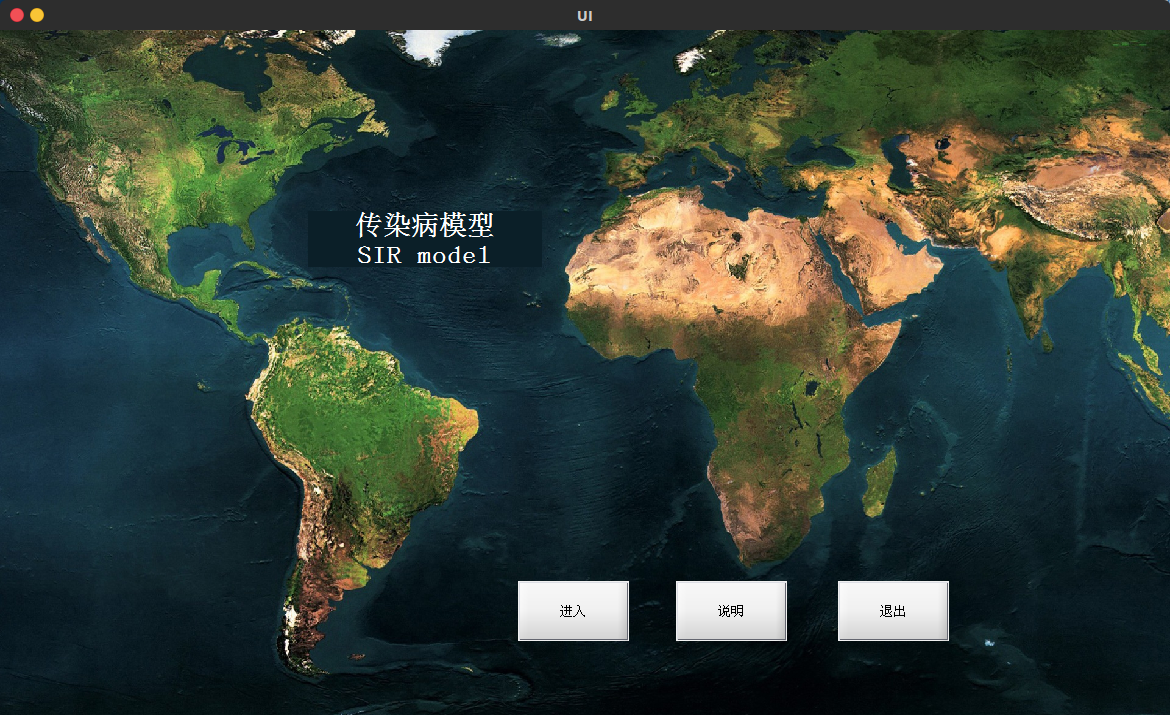
\includegraphics[scale=0.3]{Figures/UI.png}
		\caption{主界面}
	\end{figure} 
	\textbf{进入}按钮按下后立即进入仿真界面.

	\textbf{说明}按钮按下后立即进入说明界面.

	\textbf{进入}按钮按下后立即退出仿真系统.

	\subsubsection{说明界面}
	\begin{figure}[H]
		\centering
		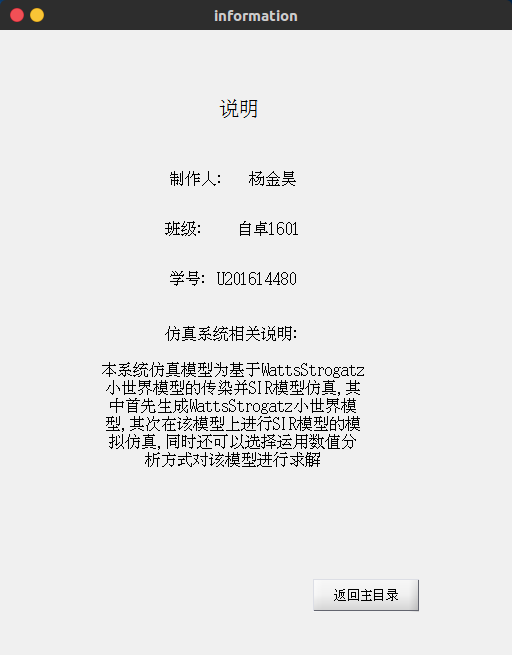
\includegraphics[scale=0.4]{Figures/info.png}
		\caption{说明界面}
	\end{figure} 
	\textbf{返回主目录}按钮按下后立即返回主界面.

	\subsubsection{仿真界面}
	\begin{figure}[H]
		\centering
		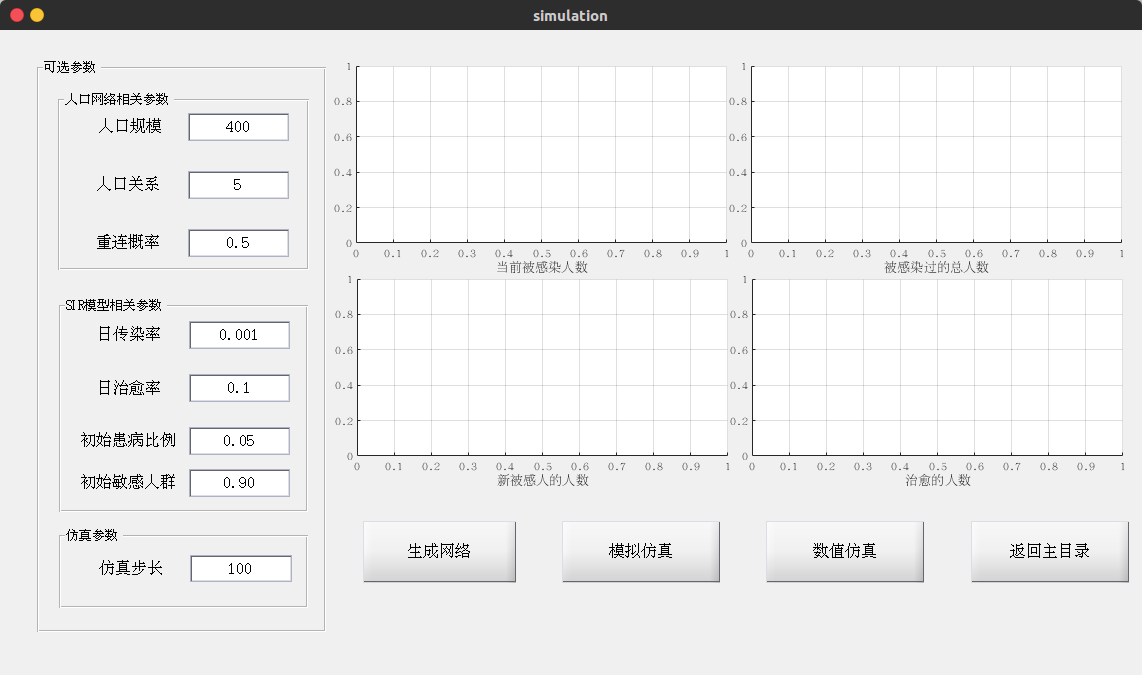
\includegraphics[scale=0.3]{Figures/simu.png}
		\caption{仿真界面}
	\end{figure} 
	左侧分别为网络模型参数,SIR模型参数和仿真参数的输入窗口 \par
	右侧为模拟仿真的结果输出. \par
	对应的按钮功能分别为: \par
	\textbf{生成网络}按钮按下后根据网络模型参数生成对应的WS小世界网络模型.\par
	\textbf{模拟仿真}按钮按下根据在WS小世界模型的基础上进行模拟仿真.\par
	\textbf{数值仿真}按钮按下后根据SIR模拟参数和仿真参数进行数值仿真.\par
	\textbf{返回主目录}按钮按下后立即返回主界面.\par

	\paragraph{注意事项}由于模拟仿真必须要在生成网络所生成的WS小世界模型进行模拟仿真,所以如要进行模拟仿真,必须先进性生成网络.同时由于网络生成时有可能会因为算量较大需要等待一段时间,可能会先显示之前的仿真网络,之后待新网络生成后界面会进行刷新.\par
	与此相比,由于数值仿真直接根据微分方程进行数值求解,所以无需进行生成网络,直接数值仿真可以得到数值仿真结果.

	\section{程序运行分析实例}
	由下图所示参数进行程序运行分析.
	\begin{figure}[H]
		\centering
		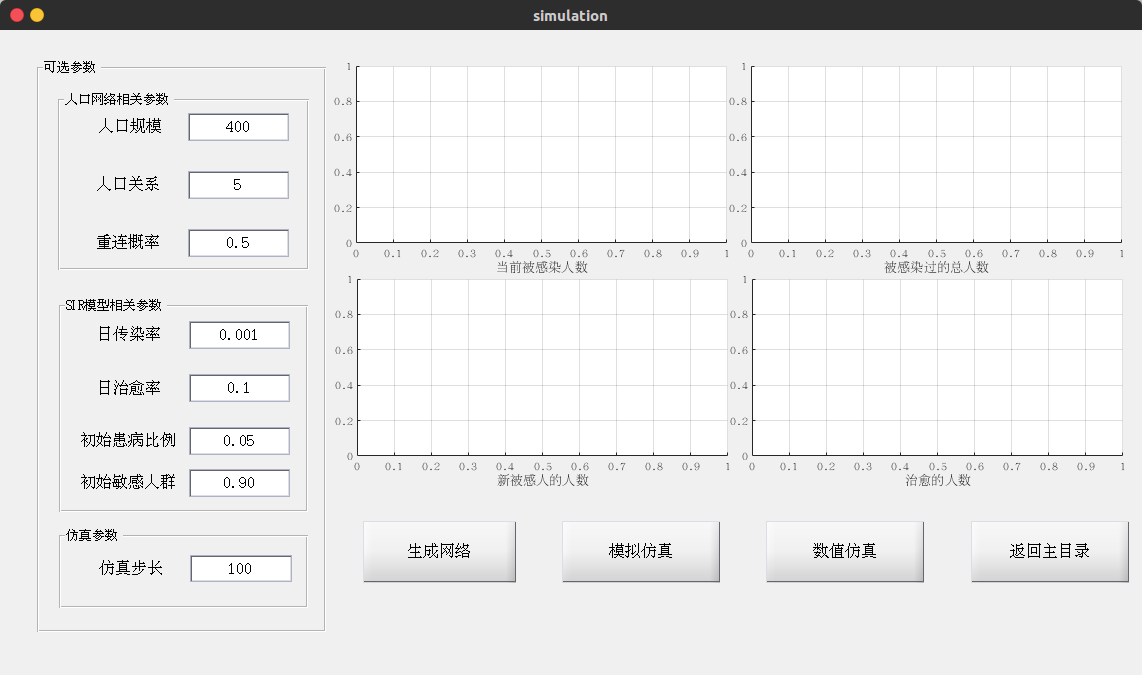
\includegraphics[scale=0.3]{Figures/simu.png}
	\end{figure} 

	\subsection{生成网络}
	\begin{figure}[H]
		\centering
		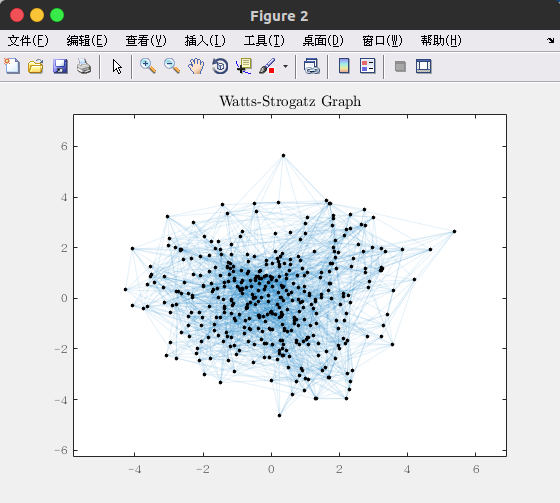
\includegraphics[scale=0.5]{Figures/net.png}
		\caption{生成网络}
	\end{figure} 
	由改图可以看出来整个网络的边连接的较为随机,可以对生成的WS小世界模型有直观的感受.

	\subsection{模拟仿真}
	\begin{figure}[H]
		\centering
		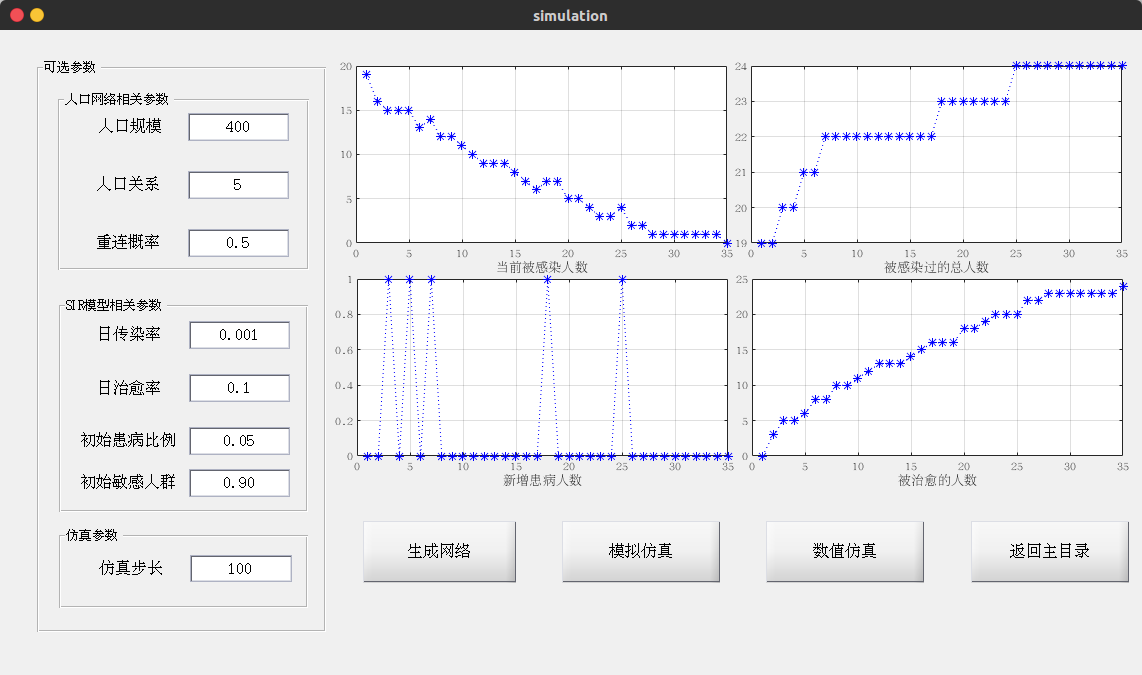
\includegraphics[scale=0.35]{Figures/moni.png}
		\caption{模拟仿真}
	\end{figure} 
	从改图中我们可以得知由于传染概率低所以该传染病很难在人群中进行传播,当时间在20天到25天时,将近90\%的人被治愈.

	\begin{figure}[H]
		\centering
		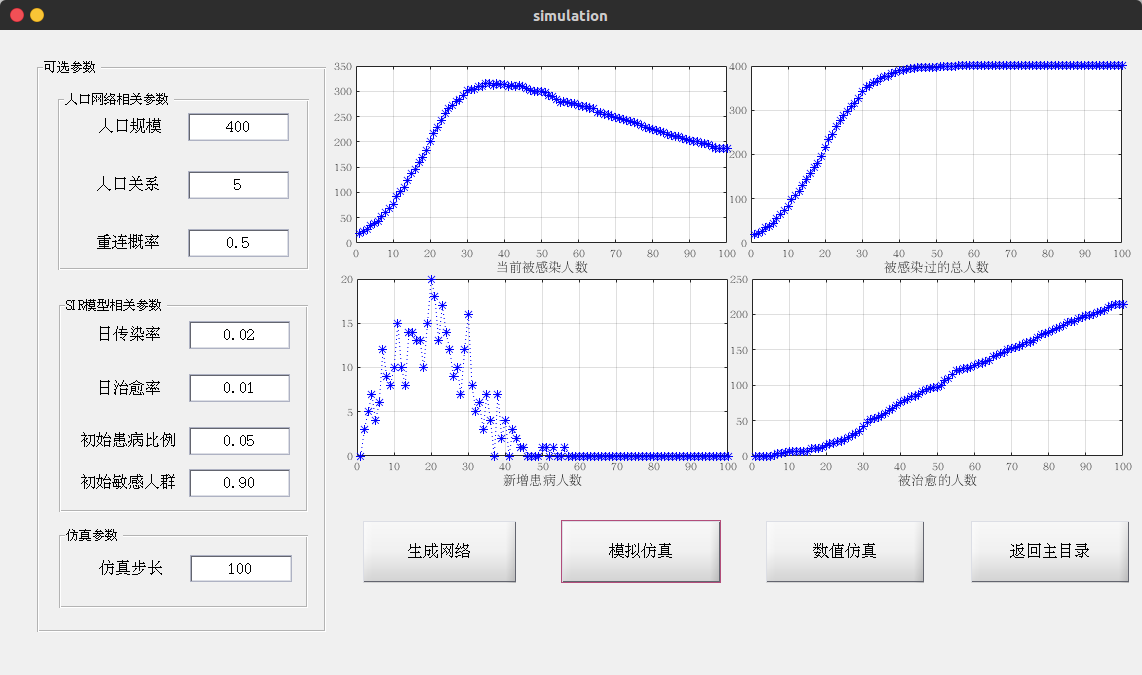
\includegraphics[scale=0.35]{Figures/moni2.png}
		\caption{模拟仿真2}
	\end{figure} 
	在修改传染率为0.02,治愈率为0.01后.传染概率的提高让仿真前期病毒被传染的可能性,由新增被感染的人数可以看出,在前期传染病广泛传播,结合当前被感染人数可得,在40-50天的时候几乎所有人群均被传染过.同时结合被治愈的人数曲线,可知患病者中被治愈的人数稳定增加,总有一天所有患病者均将被治愈.

	\subsection{数值分析}
	\begin{figure}[H]
		\centering
		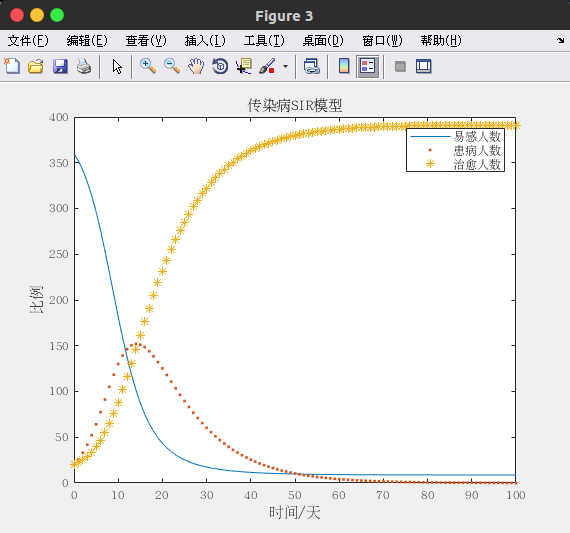
\includegraphics[scale=0.5]{Figures/shuzhi.png}
		\caption{数值分析}
	\end{figure} 
	改图为在默认参数下进行的数值仿真,从图中可以得知,易感结点敏感人群逐步减少,治愈人群稳定增加,患病者新增加后减小,其中在15天左右的时候达到峰值. \par

	\subsection{总结}
	由于数值分析是根据微分方程通过数值分析的方式求出的数值解,但这本质上是理论上的模型,而通过模拟仿真可以在一定程度上看做是真实情况的仿真,所以数值分析和模拟仿真一定会有出入,通过对比两种仿真的结果,我们可以更好的通过该模型对可治愈的传染病进行预测以及奉献的控制.

	\section{重点代码}
	\subsection{UI}
	\textbf{显示背景} \par
	\begin{lstlisting}
function figure1_CreateFcn(hObject, eventdata, handles)
pic=axes('units','normalized','pos',[0 0 1 1]);
uistack(pic,'down');
ii=imread('world.jpg');
image(ii);
colormap gray
set(pic,'handlevisibility','off','visible','off');
	\end{lstlisting}
	\textbf{不同场景的切换}\par
	\begin{lstlisting}
function pushbutton1_Callback(hObject, eventdata, handles)
close(handles.figure1);
simulation;

function information_Callback(hObject, eventdata, handles)
close(handles.figure1);
information;
	\end{lstlisting}

	\subsection{模拟仿真界面}

	\textbf{网络生成} \par
	\begin{lstlisting}
function gen_network_Callback(hObject, eventdata, handles)
H = handles.H;
k = handles.k;
beta = handles.b;
% 在新窗口进行小世界网络的展现
figure(2)
WS_world = WattsStrogatz(H,k,beta);
handles.WS_world = WS_world;
plot(graph(WS_world),'NodeColor','k','EdgeAlpha',0.1);
title('Watts-Strogatz Graph','Interpreter','latex');
guidata(hObject,handles);
	\end{lstlisting}

	\textbf{开始模拟仿真}\par
	\begin{lstlisting}
function start_Callback(hObject, eventdata, handles)
%将治愈者移出仿真总人数,并构建初始被感染者
H = handles.H*(handles.start_node+handles.sen);
p = handles.start_node;
parent_node = zeros(1,H*p);
i = 1;
[~,n] = size(parent_node);
while i <= n
r = randi([1,H]);
if (~ismember(r,parent_node))
    parent_node(i) = r;
    i = i+1;
end
end 
% SIR模型仿真
[inf,nisum,rec,infsum] = sir_simulation(handles.WS_world,...
				parent_node,...
				handles.inf_prob,...
				handles.rec_prob,...
				handles.step);
% 绘图
axes(handles.axes1);
plot(inf, 'b*:');
xlabel('当前被感染人数');
grid on

axes(handles.axes2);
plot(infsum, 'b*:');
xlabel('被感染过的总人数');
grid on

axes(handles.axes3);
plot(nisum, 'b*:');
xlabel('新增患病人数');
grid on

axes(handles.axes4);
plot(rec, 'b*:');
xlabel('被治愈的人数');
grid on

guidata(hObject,handles);
	\end{lstlisting}

	\textbf{数值分析} \par
	\begin{lstlisting}
function ode_Callback(hObject, eventdata, handles)
% 设置仿真步长,以及初始值
ts = 0:1:handles.step;
x0 = [handles.H*handles.sen,handles.H*handles.start_node,handles.H*(1-handles.start_node-handles.sen)];
%进行数值仿真
[t,x] = ode45(@(t,x) sirmodel(t,x,handles.inf_prob,handles.rec_prob), ts, x0);
%在新窗口绘图
figure(3);
plot(t,x(:,1),t,x(:,2),'.',t,x(:,3),'*');
xlabel('时间/天');
ylabel('比例');
legend('易感人数','患病人数','治愈人数');
title('传染病SIR模型');
	\end{lstlisting}

	\subsection{WattsStrogatz.m}
	\begin{lstlisting}
function h = WattsStrogatz(N,K,beta)
% OUTPUT
% H = WattsStrogatz(N,K,beta)返回由N个节点,N*K条边,节点度数2*K构造,
% 以beta概率重连边得到的WS模型
% beta = 0为圆形,beta = 1为随机图

% INPUT
% N - 结点总数
% K - 每个节点的边数
% beta - 每条边的重连概率

% 连接每个节点和他后向K临近的节点,该步骤构造结果为圆形
s = repelem((1:N)',1,K); % 源节点矩阵
t = s + repmat(1:K,N,1); % K临近目标节点矩阵,并做调整
t = mod(t-1,N)+1;

% 以beta概率重新连接每个节点对应的目标节点
% 先确定需要重连的边
% 在确定新连接的边(保证不重复)
% 在生成的网路上进行操作
for source=1:N    
    switchEdge = rand(K, 1) < beta;
    
    newTargets = rand(N, 1);
    newTargets(source) = 0;
    newTargets(s(t==source)) = 0;
    newTargets(t(source, ~switchEdge)) = 0;
    
    [~, ind] = sort(newTargets, 'descend');
    t(source, switchEdge) = ind(1:nnz(switchEdge));
end

% 将生成的网络转化为满邻接矩阵
h = full(adjacency(graph(s,t)));
end
	\end{lstlisting}

	\subsection{sir\_simulation.m}
	\begin{lstlisting}
function[inf,nisum,rec,infsum] = sir_simulation(A,parent_node,prob,r,num_of_steps)
%OUTPUT
%inf - 当前被感染的人数
%nisum - 新被感人的人数
%rec - 被治愈的人数
%infsum - 被感染的总人数

%INPUT
% num_of_steps - 最大仿真步数,如果在达到最大仿真步数之前,所有结点都被治愈将结束仿真.
% prob - 每个节点被传染的概率
% r - 治愈概率
% parent_node - 开始时刻被感染你的人数,parent_node为起始结点的ID,传染病将从其中结点进行传播
%example: parent_node = [1 5 7] 意味着传染将从 1 5 7 三个结点开始.

% 生成开始时全图的索引数组,其中x==1为被感染者,x==0为敏感人群.
num_of_nodes = size(A,1);
x = zeros(1,num_of_nodes);
x(parent_node) = 1;

all_prob = ones(num_of_nodes,1)*prob;

inf = [];
nisum = [];
r_sequence = [];

    for i = 1:num_of_steps 
        % 第一步进行初始化
        if i == 1
            z = x;
            ni = zeros(1,num_of_nodes);
            if rand<r;  ni(x==1) = 1; end
            recovered = ni';
            z_all(1,:) = z;
        else
            % 逐步模拟进行仿真
            % 获取新的总感染结点和新的被感染结点
            [z,ni] = sir_infection_step(A,z,all_prob);
            z_all(i,:) = z;
            % 获取治愈后的新的全部节点状态和新被治愈的结点
            [nA,nr] = sir_recovery_step(A,z_all(i-1,:),r);
            A = nA;
            % 统计总的被治愈的结点
            recovered = recovered + nr;
            recovered(recovered > 1)=1;
        end
        
        % 汇总当前时刻数据
        inf(i) = sum(z(z==1));
        nisum(i) = sum(ni(ni==1));
        rec(i) = sum(recovered(recovered==1));
        infsum(i) = sum(z(z==1));
        inf(i) = inf(i)-rec(i);
        
        % 感染者为0结束仿真
        if i > 1 && inf(i) == 0
            break
        end
    end
end
	\end{lstlisting}

	\subsection{sir\_infection\_step.m}
	\begin{lstlisting}
function [z,ni] = sir_infection_step(A,x0,p)
%OUTPUT
%z - output vector - 系统的新状态,1为感染者,0为敏感者
%ni - "newly infected" - 新被感染的结点列表

%INPUT
%A - 邻接矩阵
%x0 - 被感染结点的描述数组,其中1代表被感染,0代表未感染
%p - 易感结点被感染的可能性
%r_tobe - "recovered to be" - 当前步即将被治愈的结点

[~,n] = size(A);

x0(x0>1) = 1; 

% 构建概率和新感染列表
PROB = zeros(1,n);
NEWINF = zeros(1,n);

%数值调整,超过1的调整为1,尽表示是否可能被感染,
AN = sum(A(x0==1,:),1);
AN(AN>1) = 1;
SUC1 = AN;

%从新易感人群中移出已感染者
SUC = SUC1 - x0;
SUC(SUC<0) = 0;

%计算每个结点相邻的被感染者数量
NEIGH = zeros(1,n);
for i = find(SUC==1)
    AN = and(A(:,i),x0');
    NEIGH(i) = sum(AN);
end

%计算每一个结点的被传染的概率,相邻的感染者与被感染概率成指数关系
if size(p,1)==1
    for i = 1:n
        PROB(i) = 1-(1-p)^NEIGH(i);
    end
else
    for i = 1:n
        PROB(i) = 1-(1-p(i))^NEIGH(i);
    end
end

%计算新的被感染结点
for i = 1:n
    format long
    r = rand;
    if r <= PROB(i)
        NEWINF(i) = 1;
    end
end
ni = NEWINF;
%构建新的包含总的被感染者的节点列表
z = NEWINF + x0;

end
	\end{lstlisting}

	\subsection{sir\_recovery\_step.m}
	\begin{lstlisting}
function [nA,nr] = sir_recovery_step(A,z,r)
%OUTPUT
%nA - 溢出了治愈结点的新的邻接矩阵
%nr - "newly recovered" - 该步被治愈者的结点列表

%INPUT
%A - 邻接矩阵
%z - 感染结点
%r - rate of recovery - 治愈概率

remove = times(z',rand(size(z,2),1));

% 确定被治愈者
remove(remove > 1-r) = 1;
remove(remove <= 1-r) = 0;

%对邻接矩阵进行调整
A(remove == 1,:) = 0;
A(:,remove == 1) = 0;
nA = A;
nr = remove;
end	
	\end{lstlisting}

	\subsection{sirmodel.m}
	\begin{lstlisting}
% 建立SIR模型的三个常微分方程
function y=sirmodel(t,x,prob,r)
y=[-prob*x(1)*x(2),prob*x(1)*x(2)-r*x(2),r*x(2)]';
	\end{lstlisting}

	\nocite{*}

	\bibliography{Bibs/mybib}
\end{document}
